\documentclass[logo,reportComp]{thesis}
\usepackage[cpp,pseudo]{mypackage}
\usepackage{forest}

\usetikzlibrary{automata,backgrounds,fit,shapes,positioning}

\tikzset{->, % makes the edges directed
>=stealth, % makes the arrow heads bold
node distance=2.5cm, % specifies the minimum distance between two nodes. Change if necessary.
every state/.style={thick, fill=gray!10}, % sets the properties for each 'state' node
}

\title{编译原理作业六}
\subtitle{}
\school{数据科学与计算机学院}
\author{陈鸿峥}
\classname{17大数据与人工智能}
\stunum{17341015}
\headercontext{编译原理作业}

% June 3 -> June 8

\begin{document}

\maketitle

\begin{question}
考虑以下文法:
\[\begin{array}{rrll}
(1) & E &\to & E+T\\
(2) & E &\to & T\\
(3) & T &\to & TF\\
(4) & T &\to & F\\
(5) & F &\to & F^*\\
(6) & F &\to & a\\
(7) & F &\to & b
\end{array}\]
\begin{enumerate}
	\item 写出每个非终端符号的FIRST集和FOLLOW集.
	\item 构造识别这一文法所有活前缀(viable prefixes)的LR(0)自动机(参照课本4.6.2节图4.31).
	\item 构造这一文法的SLR分析表(参照课本4.6.3节图4.37).
	\item 给出SLR分析器识别输入串$a+ab^*$的过程(参照课本4.6.4节图4.38)
\end{enumerate}
\end{question}
\begin{answer}
\begin{enumerate}
	\item $FIRST$集和$FOLLOW$集如下
	\[\begin{array}{rlrl}
	FIRST(E) &= \{a,b\} & FOLLOW(E) &=\{\$,+,\}\\
	FIRST(T) &= \{a,b\} & FOLLOW(T) &=\{\$,+,a,b\}\\
	FIRST(F) &= \{a,b\} & FOLLOW(F) &=\{\$,+,*,a,b\}\\
	\end{array}\]
	\item 构造增广语法$E'\to E$,并得到LR(0)自动机如下
	\begin{figure}[H]
	\centering
	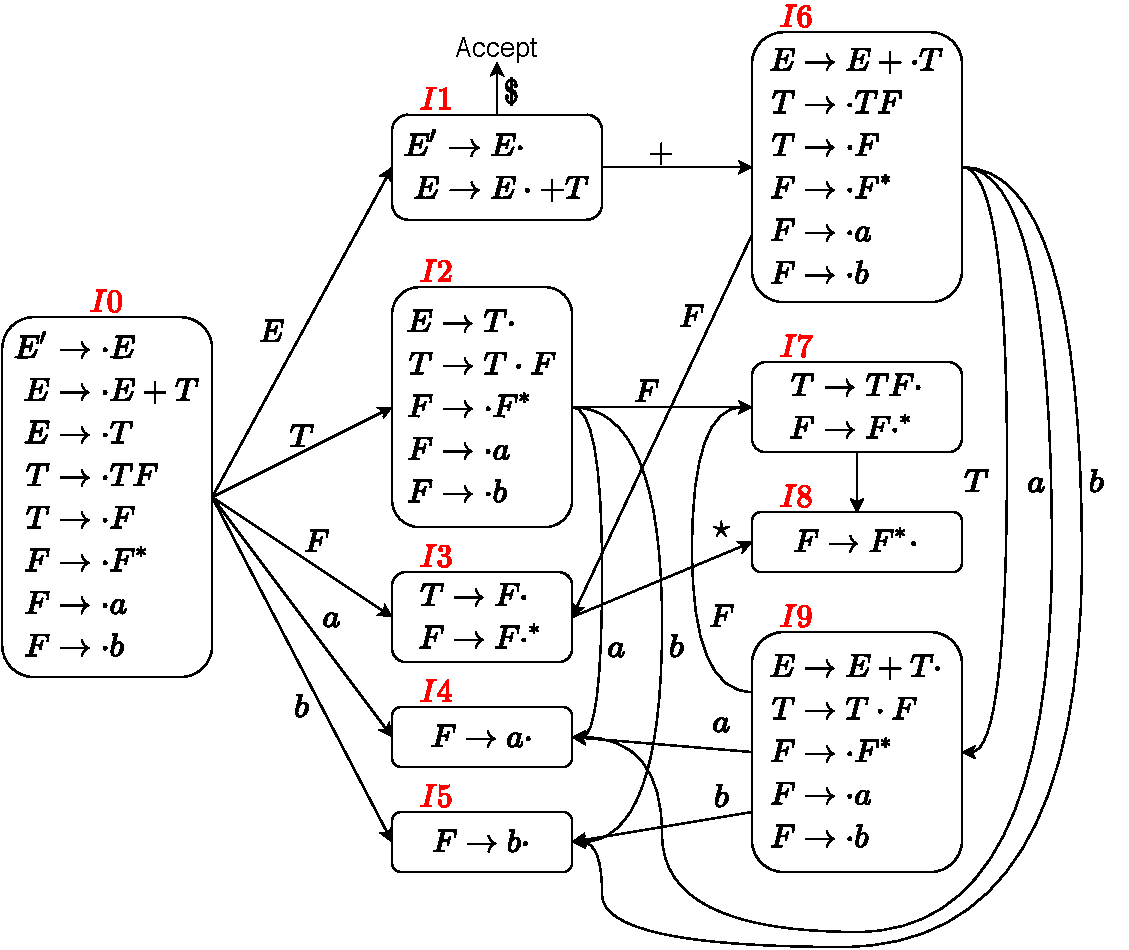
\includegraphics[width=0.8\linewidth]{fig/T06.pdf}
	\end{figure}
	\item 依据上述两问结果,可构造SLR分析表如下
	\begin{center}
	\begin{tabular}{|c|ccccc|ccc|}\hline
	\multirow{2}{*}{STATE} & \multicolumn{5}{c|}{ACTION} & \multicolumn{3}{c|}{GOTO}\\\cline{2-9}
	  & a  & b  & +  & *  & \$  & E & T & F \\\hline
	0 & s4 & s5 &    &    &     & 1 & 2 & 3 \\\hline
	1 &    &    & s6 &    & ACC &   &   &   \\\hline
	2 & s4 & s5 & r2 &    & r2  &   &   & 7 \\\hline
	3 & r4 & r4 & r4 & s8 & r4  &   &   &   \\\hline
	4 & r6 & r6 & r6 & r6 & r6  &   &   &   \\\hline
	5 & r7 & r7 & r7 & r7 & r7  &   &   &   \\\hline
	6 & s4 & s5 &    &    &     &   & 9 & 3 \\\hline
	7 & r3 & r3 & r3 & s8 & r3  &   &   &   \\\hline
	8 & r5 & r5 & r5 & r5 & r5  &   &   &   \\\hline
	9 & s4 & s5 & r1 &    & r1  &   &   & 7 \\\hline
	\end{tabular}
	\end{center}
	\item 依上述ACTION-GOTO表,可得以下过程
	\begin{center}
	\begin{tabular}{|r|l|l|r|l|}\hline
		& STACK & SYMBOLS & INPUT      & ACTION\\\hline
	(1) & 0     &         & $a+ab^*\$$ & shift\\\hline
	(2) & 04    & $a$     & $+ab^*\$$  & reduce by $F\to a$\\\hline
	(3) & 03    & $F$     & $+ab^*\$$  & reduce by $T\to F$\\\hline
	(4) & 02    & $T$     & $+ab^*\$$  & reduce by $E\to T$\\\hline
	(5) & 01    & $E$     & $+ab^*\$$  & shift\\\hline
	(6) & 016    & $E+$     & $ab^*\$$  & shift\\\hline
	(7) & 0164    & $E+a$     & $b^*\$$  & reduce by $F\to a$\\\hline
	(8) & 0163    & $E+F$     & $b^*\$$  & reduce by $T\to F$\\\hline
	(9) & 0169    & $E+T$     & $b^*\$$  & shift\\\hline
	(10) & 01695  & $E+Tb$    & ${}^*\$$ & reduce by $F\to b$\\\hline
	(11) & 01697  & $E+TF$    & ${}^*\$$ & shift\\\hline
	(12) & 016978 & $E+TF^*$    & $\$$ & reduce by $F\to F^*$\\\hline
	(13) & 01697  & $E+TF$    & $\$$ & reduce by $T\to TF$\\\hline
	(14) & 0169   & $E+T$     & $\$$ & reduce by $E\to E+T$\\\hline
	(15) & 01     & $E$     & $\$$ & accept\\\hline
	\end{tabular}
	\end{center}
\end{enumerate}
\end{answer}

\end{document}